\section{Medição da chuva}

\subsection{Pluviômetro}
As medições das precipitações de chuvas são realizadas com a utilização de um pluviômetro (Figura 1), aparelho com medidas normalizadas em formato cilíndrico que, exposto às intempéries, reserva a água da chuva precipitada entre um intervalo de leituras. Uma proveta graduada permite a leitura do volume de água acumulado dentro do medidor. O volume de água, dividido pela área de captação do pluviômetro, resulta em uma altura análoga de chuva, definida em milímetros. As leituras devem ser realizadas diariamente, sempre no mesmo horário \cite{manual-daee}.

\begin{figure}[H]
    \caption{Representação do pluviômetro}
    \centering
    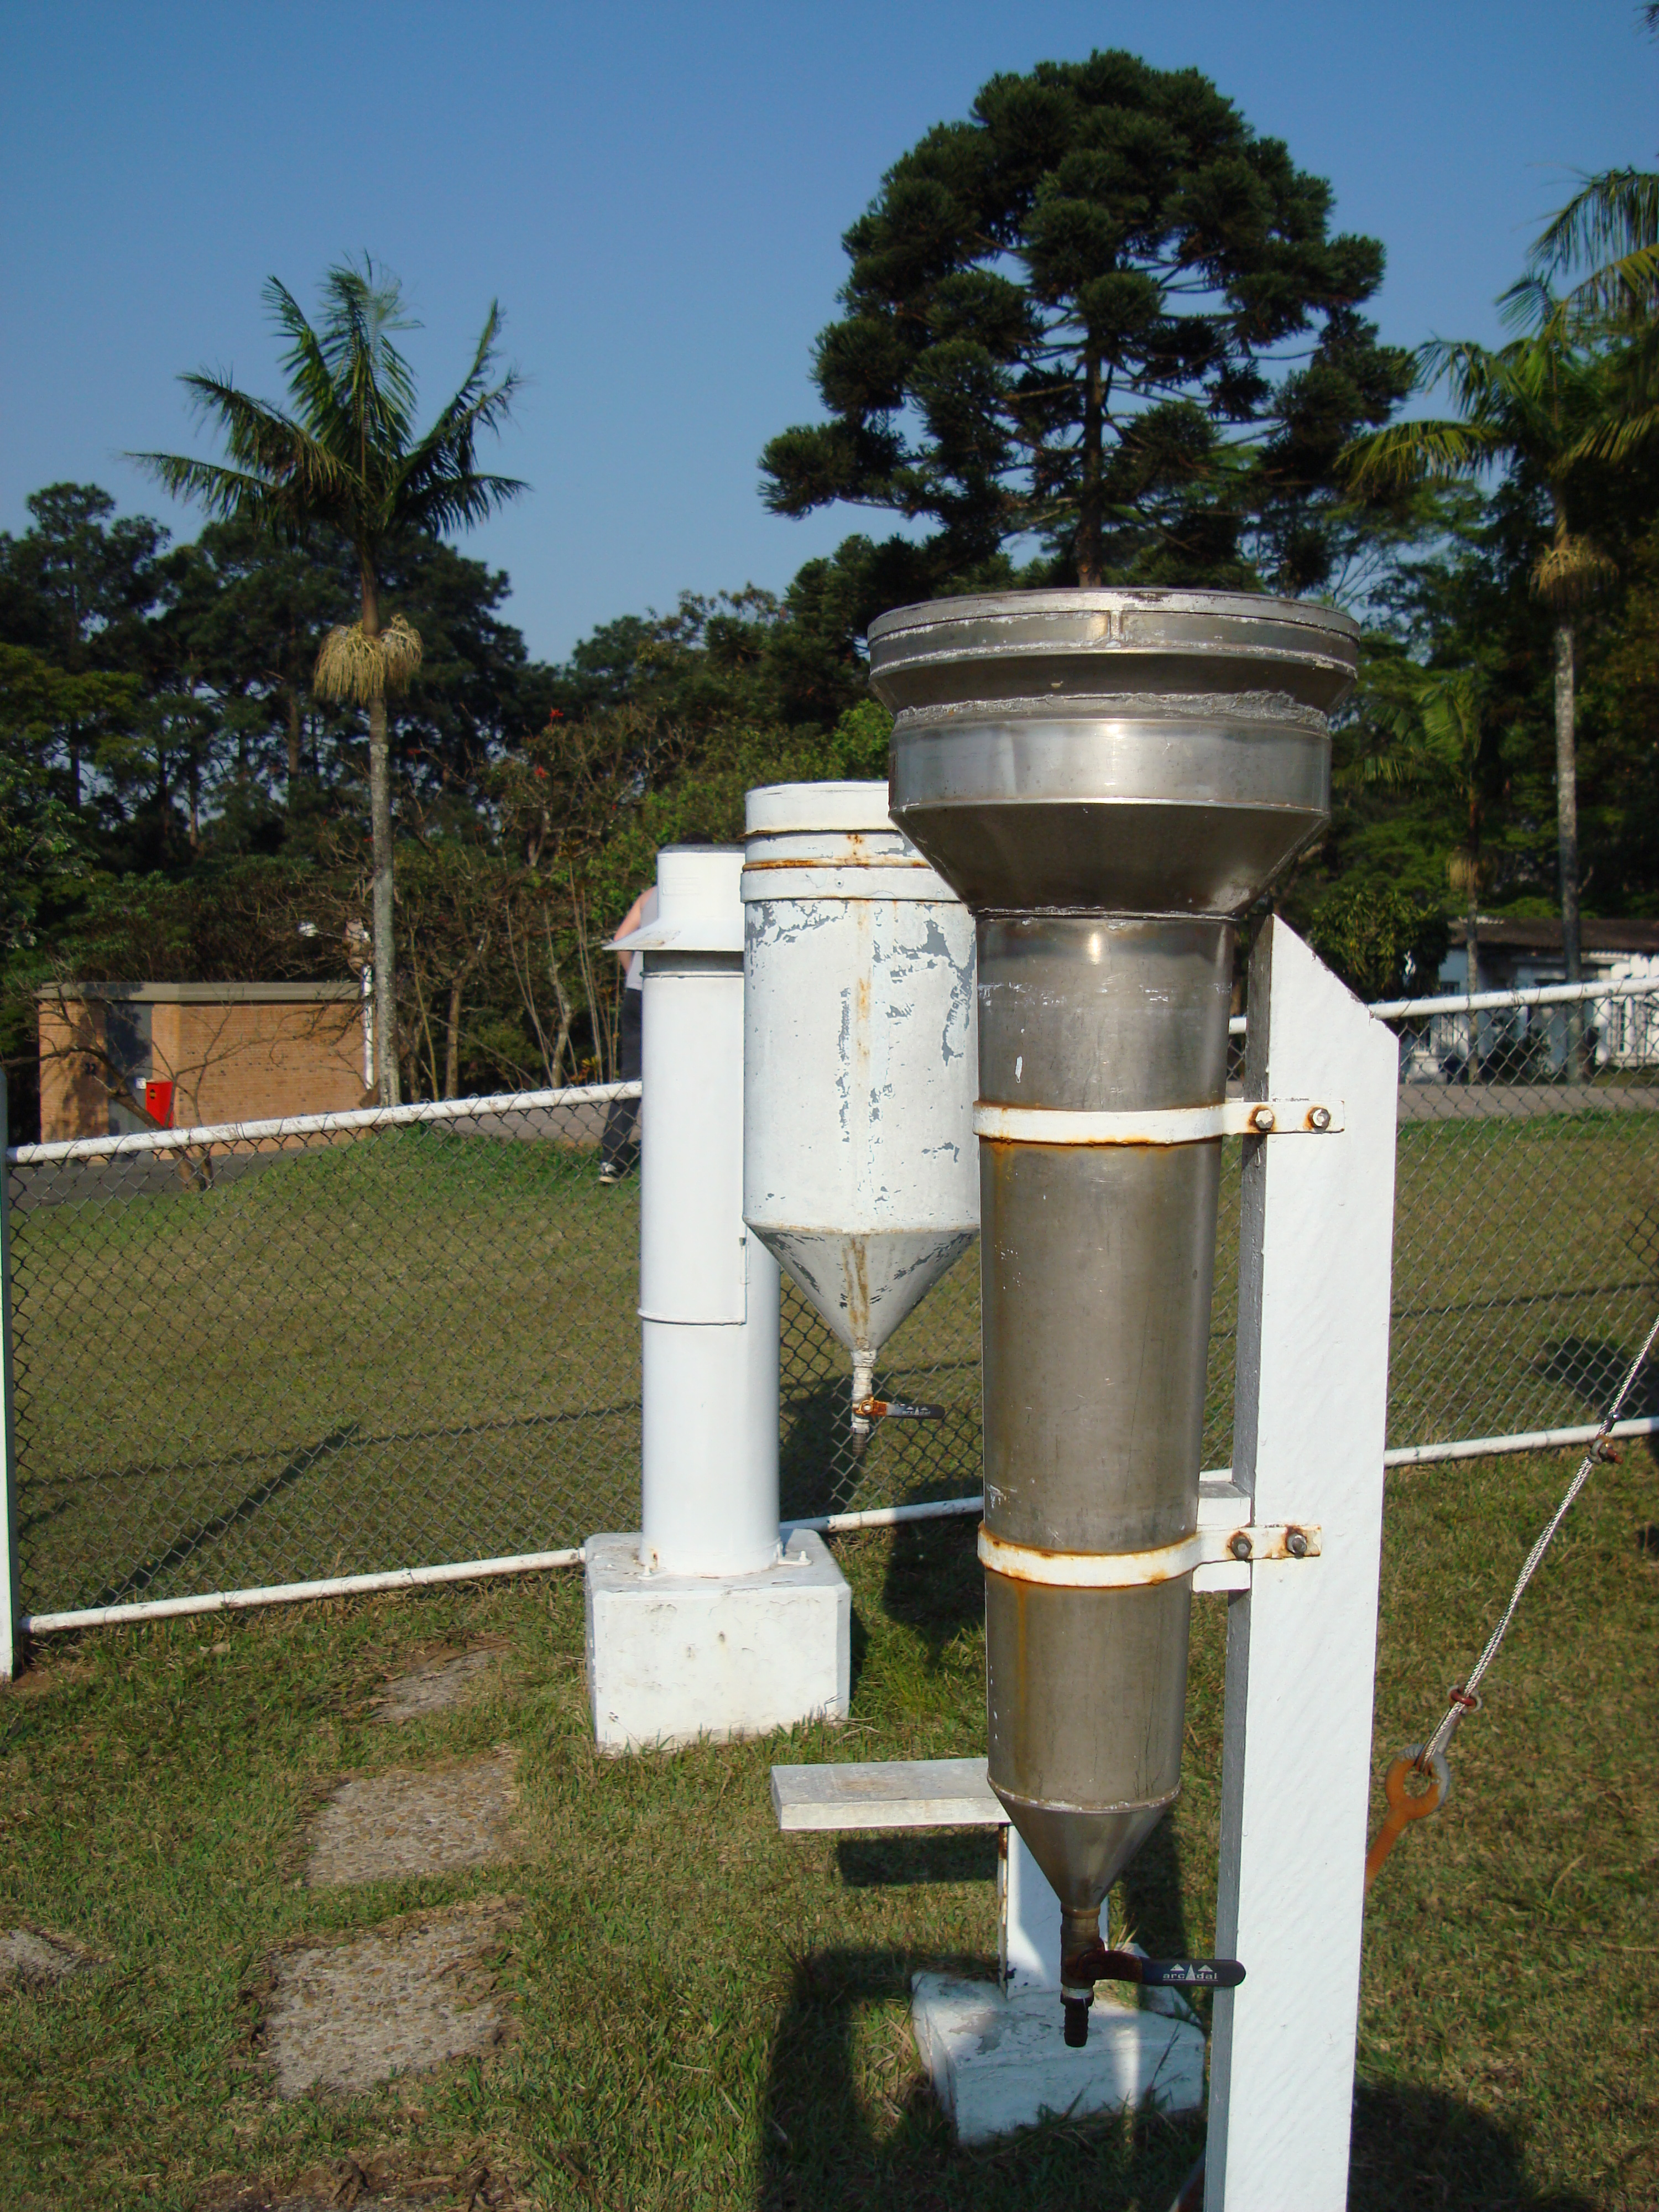
\includegraphics[width=0.25\textwidth]{Textuais/Figuras/pluviometro.jpg}
    \fonte{Autores}
    \label{fig:pluviometro}
\end{figure}


\subsection{Pluviógrafo}

Outro tipo de medidor de chuvas é o Pluviógrafo (Figura 2). Existe uma grande variedade de aparelhos, usando princípios diferentes para medir e gravar continuamente as chuvas. Os pluviógrafos permitem medir as intensidades das chuvas durante intervalos de tempo àqueles obtidos com as observações manuais feitas nos pluviômetros \cite{tucci1993}.

\begin{figure}[H]
    \caption{Representação do pluviógrafo}
    \centering
    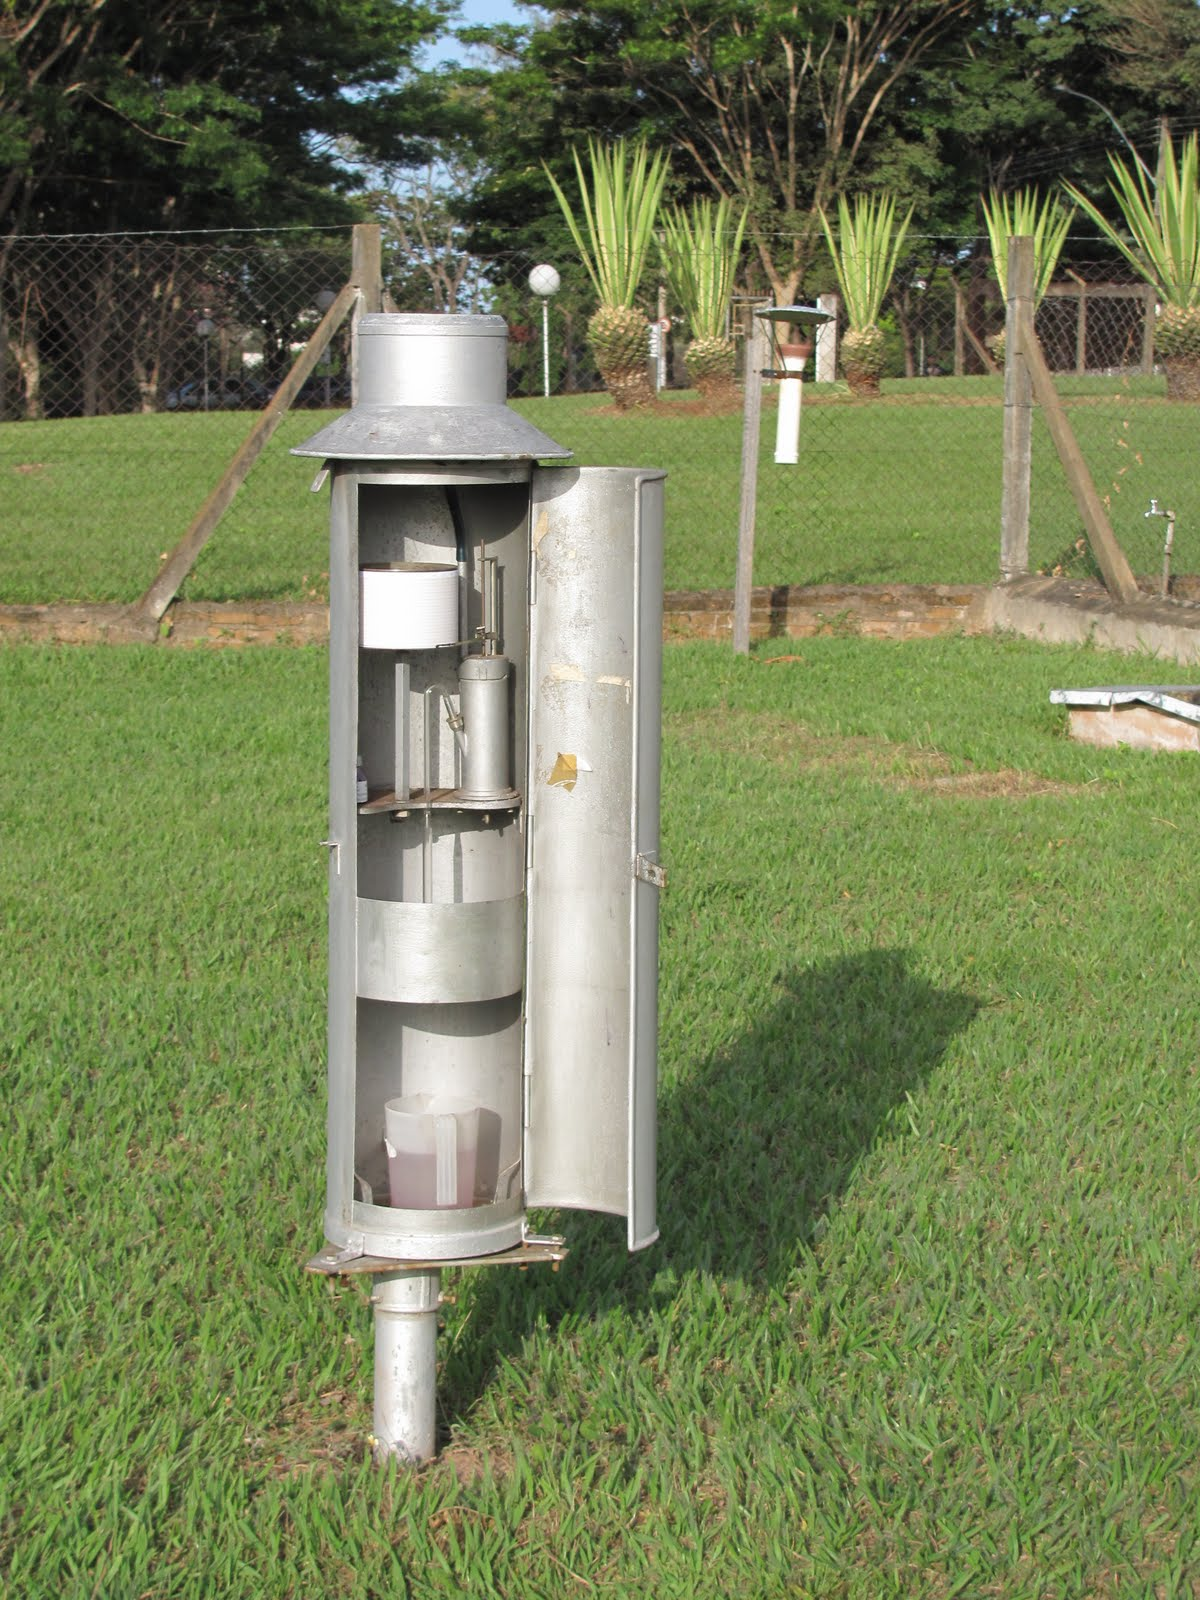
\includegraphics[width=0.5\textwidth]{Textuais/Figuras/pluviografo.jpg}
    \fonte{Autores}
    \label{fig:pluviografo}
\end{figure}

\section{Dados de chuvas no Brasil}

A Agência Nacional de Águas (ANA) disponibilizada uma relação dos postos pluviométricos instalados e operandos em todo o território brasileiro e os respectivos dados de chuva. Estas informações podem ser obtidas pela Internet por meio do Sistema de Informações Hidrológicas (HidroWeb). 

É importante destacar que, deve-se conhecer a qualidade dos dados que estão sendo utilizados, pois isso pode avariar a qualidade dos resultados dos estudos hidrológicos. Tratando-se de projetos em área urbana, recomenda-se que seja instalado ao menos um pluviógrafo, para aumentar a qualidade dos estudos hidrológicos que apoiarão, por exemplo, os projetos de controle de inundação \cite{tucci1993}.